\documentclass[11pt,a4paper,bibliography=totocnumbered]{scrartcl}
\usepackage[utf8]{inputenc}
\usepackage[british]{babel}
%\usepackage{amsmath}
%\usepackage{amsfonts}
%\usepackage{amssymb}
\usepackage[footsepline]{scrlayer-scrpage}
\usepackage{tabu}
\usepackage{placeins}
%\usepackage{longtable}
\usepackage{multirow}
\usepackage{setspace}
%\usepackage{graphicx}
%\usepackage{pgfplots}
\usepackage{hyperref}
\usepackage{url}
\usepackage{titling}
\usepackage[backend=biber,sorting=none]{biblatex}
\usepackage{csquotes}
\usepackage{pdfpages}
\usepackage{epstopdf}
\usepackage{graphicx}
\usepackage{subfig}
\usepackage{array}
%\usepackage{enumitem}

%\pgfplotsset{width=12cm,height=6cm,compat=1.11}

% Constants
\def\mytitle{Tomcat Native 2}
\def\myauthor{Jocelyn Thode and Simon Brulhart}
\def\theclient{Red Hat}

\pagestyle{scrheadings}

\ihead{\mytitle}
\chead{}
\cfoot{}
\ifoot{Initial plan}
\ofoot{\thepage}

\posttitle{\end{center}\begin{center}\LARGE Initial plan\end{center}}

\author{\myauthor\\ \href{mailto:jocelyn.thode@unifr.ch}{jocelyn.thode@unifr.ch} \\ \href{mailto:simon.brulhart@unifr.ch}{simon.brulhart@unifr.ch}}
\title{\huge \textbf{\mytitle}}

\bibliography{initial_plan}

\begin{document}

\graphicspath{{figures/}}

\begin{titlingpage}

\maketitle

\begin{abstract}
\mytitle{} is a project mandated by Red Hat. It aims at providing a JNI wrapper for OpenSSL for use in both Undertow and Tomcat. This project is the practical part of the R\&D Workshop course given at the University of Neuchâtel as part of the Joint Master in Computer Science.
\end{abstract}

\begin{figure}[b]
\centering
\subfloat{
\includegraphics[height=1.8cm]{unine.eps}}
\qquad
\subfloat{
\includegraphics[height=1.5cm]{jmcs.png}}
\qquad
\subfloat{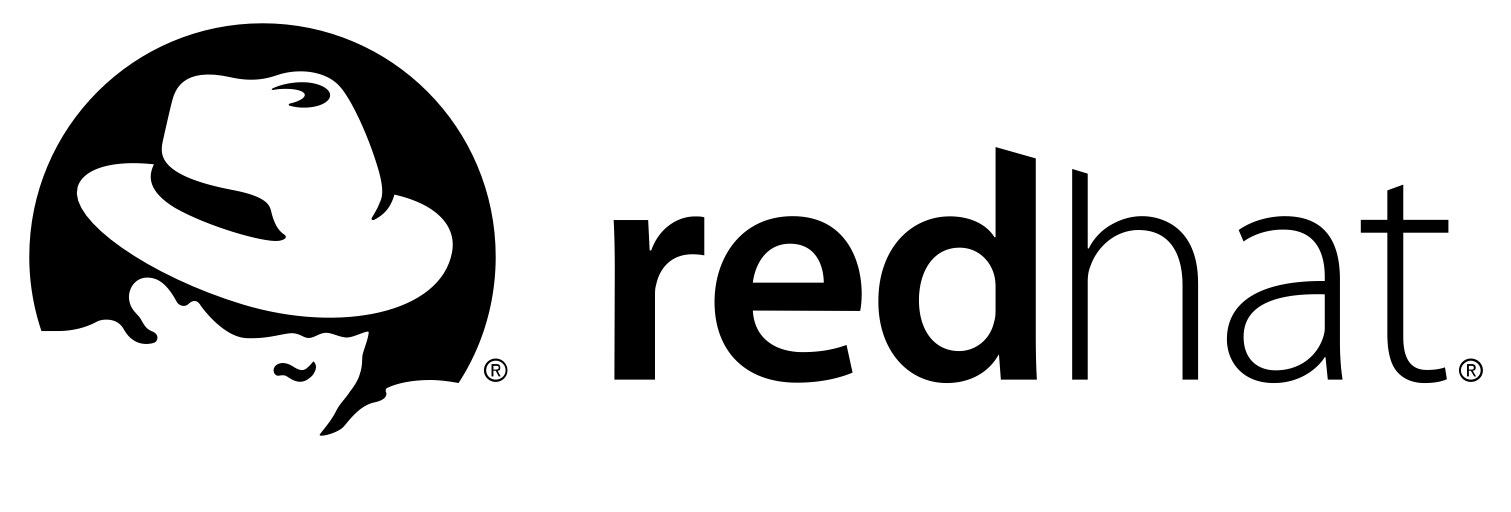
\includegraphics[height=1.6cm]{redhat-logo.png}}
\end{figure}

\end{titlingpage}

\pagebreak

\setcounter{tocdepth}{2}
\tableofcontents
\listoffigures

\pagebreak

\section{Project description}

\subsection{Project context}
For this project we are working with \theclient{} which is a multinational software company that provides open-source software and technical support to enterprises\autocite{redhat}.
At the moment, the two biggest Java web servers are Tomcat\autocite{tomcat} and Undertow\autocite{undertow}. Both rely on TLS/SSL to encrypt and secure communications between a client and a server. To achieve good performance Tomcat Native\autocite{tomcat-native} provides access to OpenSSL in Tomcat. It uses Apache Portable Runtime (APR) to do so. 
Unfortunately, Undertow isn't compatible with Tomcat Native at the moment.
Until last year, the APR would manage the encrypted sockets by itself. However this implied a lot of C code to maintain. To ease maintenance, some work has been done to use OpenSSL APIs directly instead. This works well enough despite some acceptable performance penalty. However the APR still provides the bindings to these APIs.
We now want to strip the current solution of the APR and make the result compatible with Undertow.

Figure \ref{fig:current} shows an overview of the different way to use TLS/SSL in Tomcat. This figure describes the path taken by a piece of data, going from Tomcat/Undertow to the OS network layer. There is a different color for each way to use TLS/SSL.

\subsection{Goals and objectives of the project}

Our project aims to refactor Tomcat Native to drop APR and only rely on our own JNI wrapper to interface with OpenSSL. This should make Tomcat Native much more maintainable while keeping great performance when using TLS/SSL. The project also aims to make the resulting \mytitle{} usable in Undertow while keeping the compatibility with Tomcat.
This means we need to :
\begin{enumerate}
\item Study the source code of Tomcat Native, Undertow and some experiments already done to use OpenSSL in Undertow.
\item Remove all APR code present in Tomcat Native
\item Abstract Tomcat Native to be used in Tomcat and Undertow
\item Provide good documentation so that the open-source community can use the project
\item Run benchmarks to test the implementation on multiple platforms
\item Extend the OpenSSL support by adding JNIs for more features
\end{enumerate}

Figure \ref{fig:goal} shows what is expected at the end of the project.

\section{Project organization}
\label{sec:org}

This project requires us to read some documentation and source code. We also need to write reports and presentations. To keep the code base clean, we decided to adopt the same strategy as Numa de Montmollin last year and split our work in two different repositories on Github.

\href{https://github.com/jocelynthode/tomcat-native2-doc}{tomcat-native2-doc} is the repository documenting the progress of our project. We put every report and presentation in the repo. This repo also contains a wiki which hosts the logbook, work plan and our different articles. The articles are useful to share our findings and more importantly not to forget about them.

\href{https://github.com/jocelynthode/tomcat-native2}{tomcat-native2} is the repository dedicated to the code. This repo includes our implementation, and the documentation directly concerning it. For example, it should contain a ReadMe describing the building process and the main purpose of the project.

\subsection{Responsibility distribution}

\begin{description}
\item[Jocelyn Thode] Student working on the project.\\
\href{mailto:jocelyn.thode@unifr.ch}{jocelyn.thode@unifr.ch}

\item[Simon Brulhart] Student working on the project.\\
\href{mailto:simon.brulhart@unifr.ch}{simon.brulhart@unifr.ch}

\item[Jean-Frederic Clere] Project supervisor at \theclient{}. \\
\href{mailto:jfclere@redhat.com}{jfclere@redhat.com}

\item[Rémy Maucherat] Co-Supervisor at \theclient{}.\\
\href{mailto:rmaucher@redhat.com}{rmaucher@redhat.com}

\item[Stuart Douglas] Works at \theclient{}.
Developer on Undertow.\\
\href{mailto:sdouglas@redhat.com}{sdouglas@redhat.com}

\item[Dr. Hugues Mercier] Workshop coordinator.\\
\href{mailto:hugues.mercier@unine.ch}{hugues.mercier@unine.ch}
\end{description}

As our project involves reading a lot of source code and removing code. We usually work together, sharing our findings. We meet most of the time using VoIP software and assign the tasks of the day from there. If we have any question we can always contact each other on the spot.

\subsection{Interactions with the client}

As we have to work with Stuart Douglas for Undertow who lives in Australia, Rémy Maucherat for Tomcat who lives in France and Jean-Frederic Clere who works in Neuchâtel we usually interact by email, or Hangout if we want a spoken conversation. 

We also write a logbook of our daily activity as well as some articles on our understanding of the project on Github, so that Jean-Frederic Clere and Rémy Maucherat can follow our progress.

\section{Methodology}

For this project we do not have any choice in the technology used. We work with Java and specifically JNI. We have to modify Tomcat Native so that it works with both Tomcat and Undertow without APR.

As stated earlier, we almost always get together on a VoIP chat room so that we can easily and quickly share our findings and ask questions to each other. Otherwise we try to make a work plan for the day and then split the tasks evenly from there.

We mostly use Intellij IDEA for our development environment. We use git coupled to Github as the source version control. We may also use Github issues in the future to track problems we may encounter during the implementation.

Every source code we use is free (as in freedom). They are licensed under the Apache License 2.0. Our work is completely open-source as required by Red Hat and will probably be under the Apache Licence 2.0 as it is a fork of Tomcat Native.
\subsection{State of the art}

See figure\ref{fig:current} for a visual representation.

At the moment, only Tomcat has access to OpenSSL through its library Tomcat Native. Unfortunately Undertow has to rely on the SSL implementation given by JSSE to provide SSL/TLS support. This leads to bad performance in Undertow.

On the other hand, Tomcat through Tomcat Native uses APR to access OpenSSL which is not ideal as this adds a lot of C code to maintain and isn't that useful anymore.

Our project should streamline Tomcat Native so that it can be used in both Undertow and Tomcat, giving access to a high-performance implementation of TLS/SSL to Undertow while making it easier to maintain the source code for  Tomcat as well.



\section{Constraints and elements of risk}

\subsection{Constraints}
\label{subsec:constraints}

The main constraint of our project is that everything must be open-source. This forces us to have really good documentation as our source code is completely visible and will be used by the community afterwards.

An other constraint is the fact that we have to work with people all around the world. This can create some problems when waiting on answer because of timezone differences.

\subsection{Risks}
\label{subsec:risks}
We have three main risks in our project:
\begin{enumerate}
\item Having to understand projects such as Tomcat, Tomcat Native and Undertow is a big task. We could get lost reading code and documentation for hours without really understanding anything.

\textit{However, we can always ask Rémy, Jean-Frederic and Stuart for help if we are stuck on a particular problem as we already did multiple times. Since the projects are open source we can also rely on the community to provide us documentation and help.}

\item Evaluating the time needed to adapt Tomcat can be deceptive as we have to remove code instead of writing it. This could lead to some conflicts where we remove too much or not enough or we simply don't know what to remove to make it effective.

\textit{Stuart has already done some experiments with Undertow which can help us visualize what to remove. Having our work plan checked by Rémy and Jean-Frederic can also help us in that regard.}
\item Adapting Tomcat Native to work with both Undertow and Tomcat might not be the best solution. An other approach could be to use the code written by Stuart Douglas for Undertow and modify it to work with Tomcat. This would require us to write a lot more code than the Tomcat Native route and could make us lose a lot of time if we don't choose the right alternative at the beginning.

\textit{Rémy and Jean-Frederic think that the Tomcat Native route is the easiest and we agree. Removing code is almost always easier than writing it.}
\end{enumerate}


\section{Deliverable goods}

At the end of the project we will deliver an OpenSSL wrapper using JNI calls based on Tomcat Native and working with both Tomcat and Undertow as well as documentation for this wrapper.

These will be delivered on Github in the repository presented in chapter 2. This should help the community understand our project and continue working on it.

\section{Efforts and schedule}
The full work plan and its associated logbook is available on the documentation repository referred in chapter \ref{sec:org}. We also reproduced it in Figure \ref{fig:workplan}

Our project is split up along the fixed deadlines/tasks specified by the R\&D Workshop :
\begin{itemize}
\item \textbf{Deadline 1} is the deadline concerning this report. It defines what has to be done for the project as well as reading documentation.
\item \textbf{Deadline 2} focuses on removing APR from Tomcat Native. 
\item \textbf{Deadline 3} focuses on making \mytitle{} working on both Tomcat and Undertow.
\item \textbf{Deadline 4} aims at extending OpenSSL support in \mytitle{}.
\end{itemize}

Each task is defined more precisely in the next sub-chapters.

\subsection{Task 1}
\label{subsec:task1}
The first task is entirely dedicated to understand what  is expected of us and how the different projects such as Tomcat Native work. Reading documentation will be done throughout the entire project, but here it is especially important as we have to understand the main concepts.

This deadline finishes with the hand-in of this plan. The project is on good tracks at the moment.
\subsection{Task 2}
\label{subsec:task2}

In this second task, we want to understand more precisely what is needed to keep the OpenSSL engine for JSSE working.

We then will write JNIs for OpenSSL to replace the ones from the APR. At this point we won't need the APR anymore, so we will completely remove it from the Tomcat Native code base. This task should be done by the 10th April 2016.

\subsection{Task 3}
\label{subsec:task3}

At the end of the third task, we aim at having a fully working \mytitle{} for both Tomcat and Undertow. To achieve this goal we need to understand thoroughly how the JSSE SSL Engine and Java sockets are used in both web servers as well as understand how the JSSE OpenSSL engine works in Tomcat and how could we modify it to make it work in Undertow.

\subsection{Task 4}
\label{subsec:task4}

Finally, we will have to benchmark \mytitle{} with Red Hat to see how it behaves in different conditions. Then, if time permits, we will implement more features in \mytitle{} regarding OpenSSL. For example, implementing support the OpenSSL handshake callback would be really useful as right now we have to rely on a hack to know when the handshake is completed.

Implementing support for proprietary large frames would also more performance on some systems.

Finally, implementing different security options for OpenSSL would also be a possibility.
\newpage
\printbibliography

\begin{figure}[!h]
\begin{center}
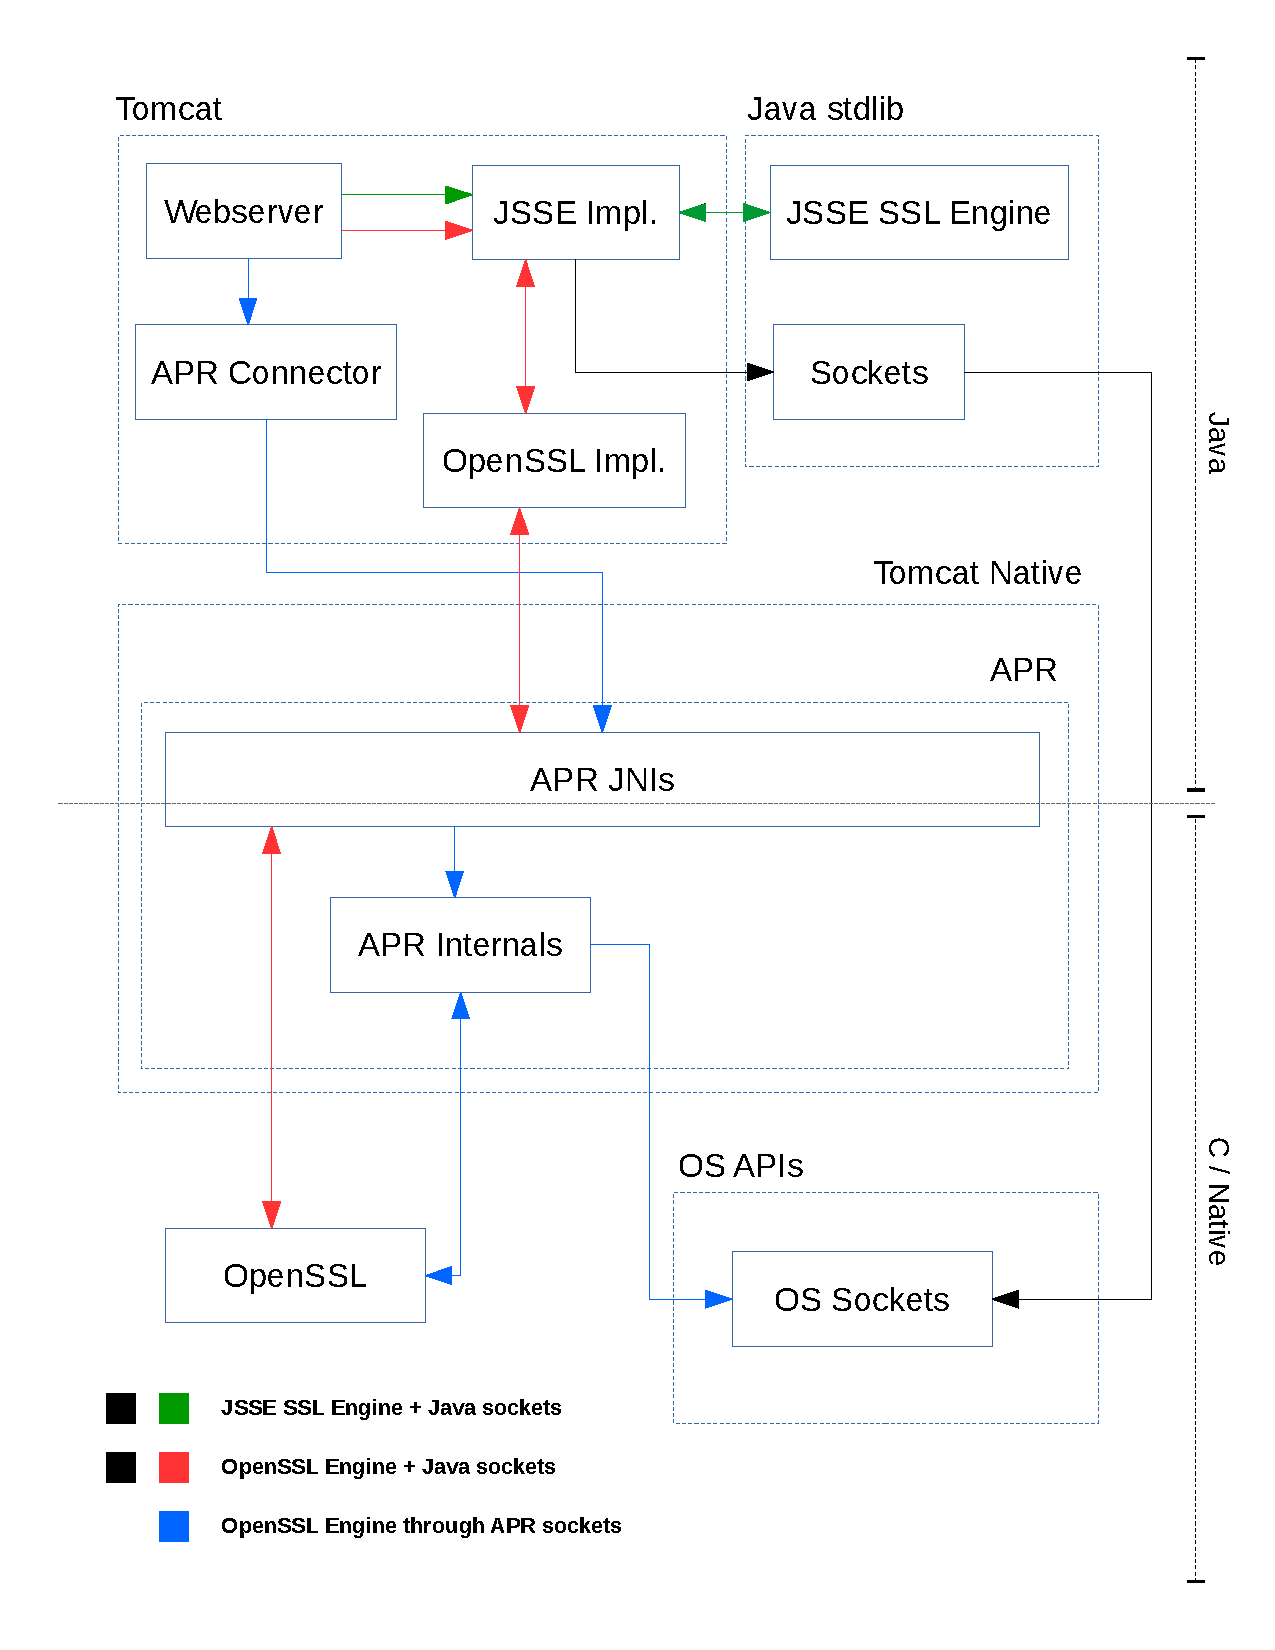
\includegraphics[scale=0.7]{diagram_current_way.pdf}
\end{center}
\caption{\textbf{Diagram showing the different ways to use TLS/SSL in Tomcat.}}
\label{fig:current}
\end{figure}

\begin{figure}[!h]
\begin{center}
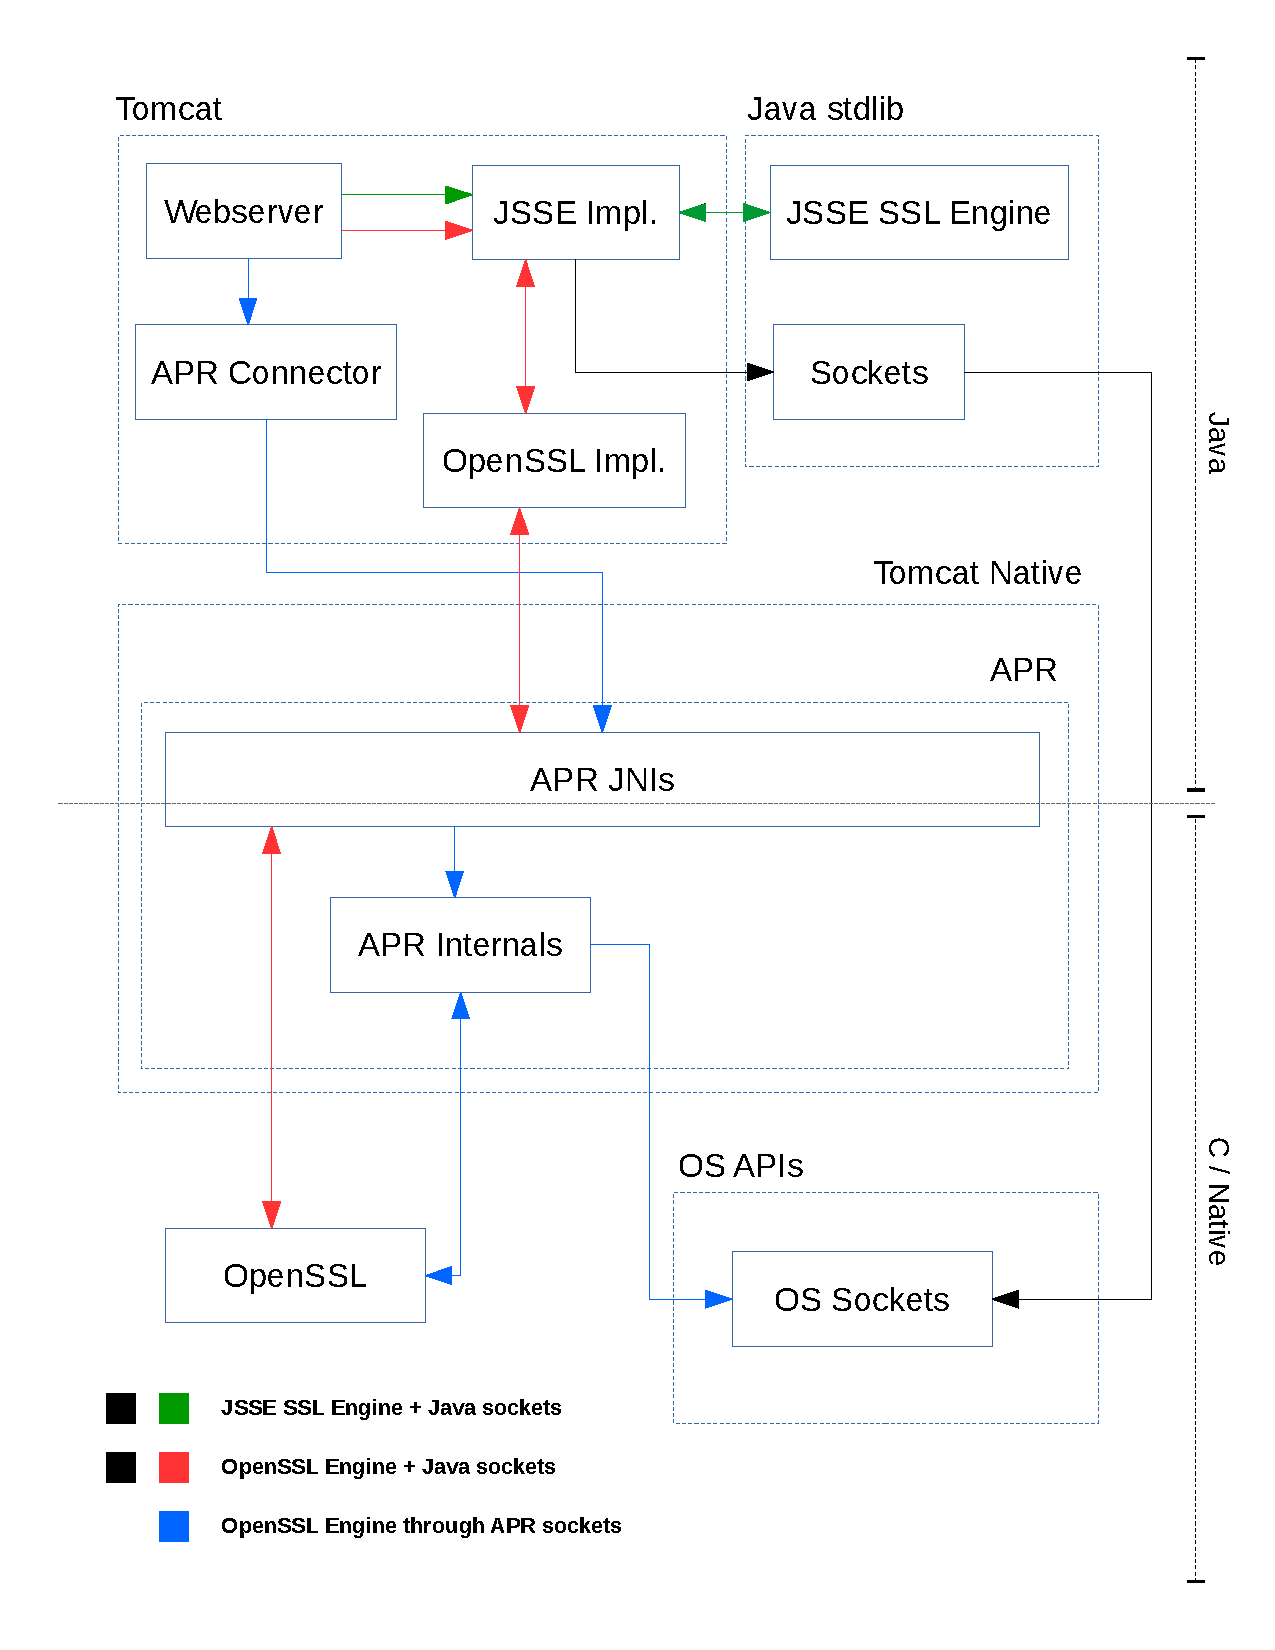
\includegraphics[scale=0.7]{diagram_goal.pdf}
\end{center}
\caption{\textbf{Diagram showing the expected end result of our project.}}
\label{fig:goal}
\end{figure}


\begin{figure}[h!]
\begin{center}
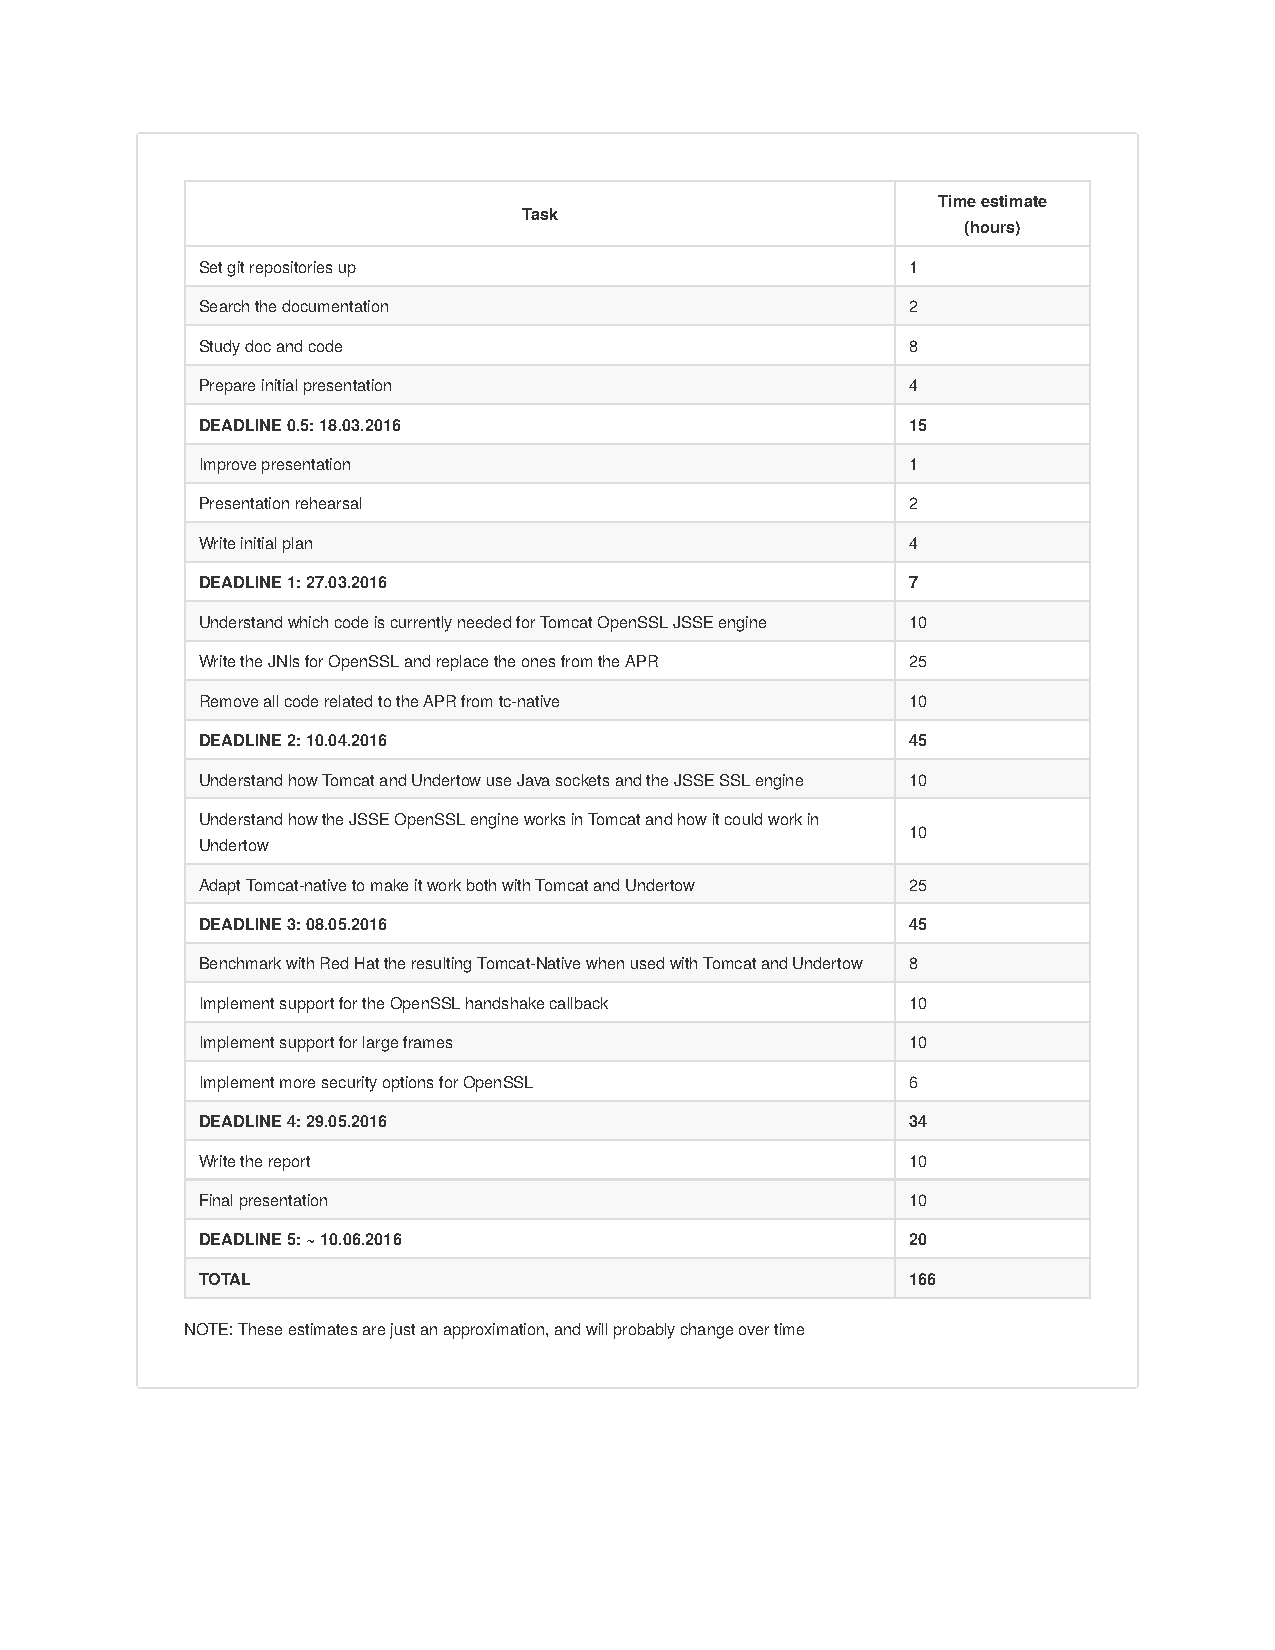
\includegraphics[trim=400 0 400 0,scale=0.9]{workplan}
\end{center}
\caption{\textbf{Workplan table from the wiki}}
\label{fig:workplan}
\end{figure}

\FloatBarrier

\end{document}